\newpage
\phantomsection
\chapter{Introduction}\label{chap:intro}

Light-matter interaction have become an important tool in medical sciences and biology, leading to the creation and development of a specialized field known as \textit{biomedical optics} or \textit{biophotonics} oriented to fundamental research, imaging, diagnosis, therapy and monitory of diseases and surgery assistance~\cite{Keiser2016_Biophotonics}. Many imaging techniques have emerged to cover the general necessity to visualize internal structures of tissues. In particular, \textit{Optical Coherence Tomography} (OCT) has become an important imaging modality for biomedical optics and medicine~\cite{Keiser2016_Biophotonics, Fujimoto2015_Optical}. A general introduction to the operation and applications of OCT in medicine is given in the following sections.

\section{Optical coherence tomography in medicine}

OCT \textit{is an imaging technique that produces three-dimensional, micrometric-resolution images of scattering samples such as biological tissues by measuring the light that is backscattered by the sample using low-coherence interferometry}~\cite{Huang1991_Optical, Fujimoto2015_Optical}.

Research community in biophotonics has shown great interest in OCT given its unique features such as high sensitive that allows to obtain useful information from biological samples with different optical properties, and its resolution of 1-15~$\mu$m and axial range of $\sim$2~mm that fills a gap between other medical imaging modalities such as ultrasound and confocal microscopy~\cite{Fujimoto2015_Introduction}. Furthermore, non-invasive operation of OCT, both \textit{ex vivo} and \textit{in vivo}, with no contrast agents nor ionizing radiation are important features that have positioned OCT in the medical community for imaging of tissue pathologies \textit{in situ} and in real time, particularly in ophthalmology~\cite{Swanson1993_vivo, Schuman2004_Optical}, but also in endoscopic imaging~\cite{Tearney1997_vivo}, intravascular imaging~\cite{Tearney1996_CatheterBased, Bouma2017_Intravascular} and dermatology~\cite{Welzel1997_Optical, Olsen2018_Advances} among others~\cite{Colston1998_Imaging, Suter2012_Optical, Vakoc2012_Cancer}.

OCT produces cross-sectional and volumetric images by measuring the magnitude and ``echo time delay'' of light backscattered by the sample~\cite{Huang1991_Optical}, similarly to the operation of other tomography techniques, such as ultrasound~\cite{Hoskins2019_Diagnostic} that employs sound instead of light. Backscattered light contains information of the optical properties of the sample and this information can be distinguished at different depths by determining the time it takes for light to travel different axial distances, thus performing an axial scan that can be expanded to a cross-sectional image (as depicted in Figure~\ref{fig:BasicOCT}) and also to volumetric images. Given the large magnitude of speed of light of $\sim$3x10$^8$m/s, there are technical limitations to make electronic devices with the required sensitivity and time resolution to measure the echo time delay of light with micrometric resolution~\cite{Fujimoto2015_Introduction}. Hence, OCT employs low-coherence interferometry to measure the backscattered light in terms of optical path length differences rather than measuring directly the temporal delays~\cite{Huang1991_Optical}, being both related through the speed of light.

\begin{figure}
    \centering
    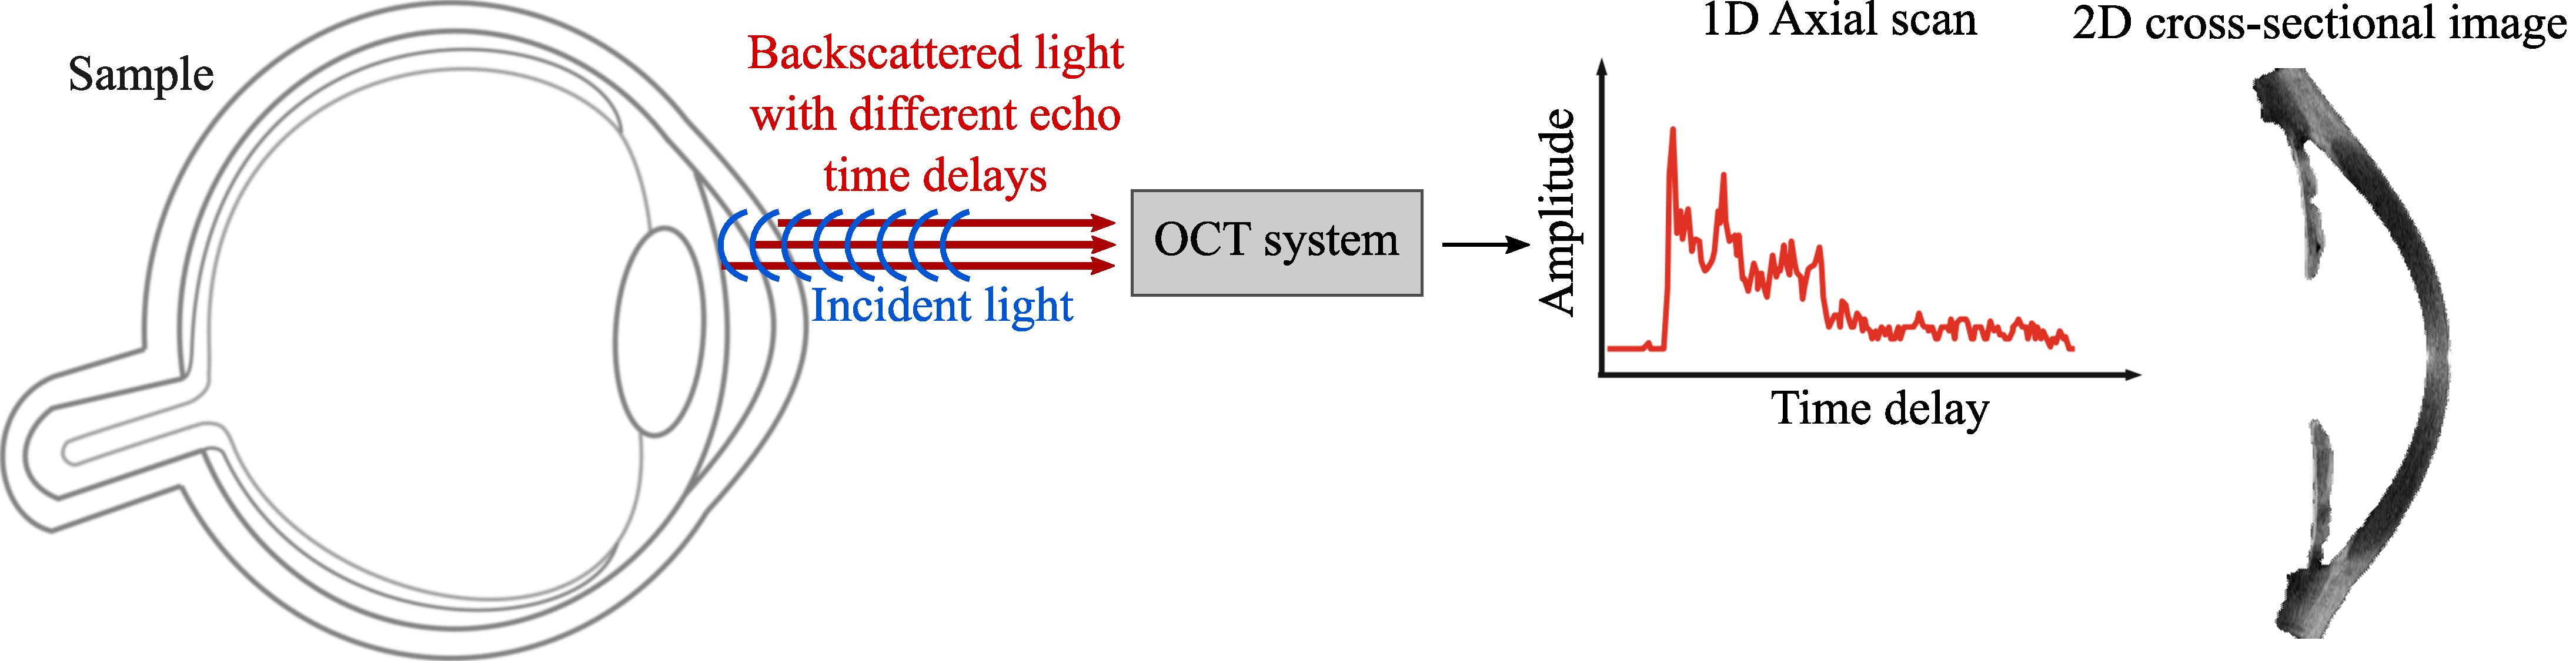
\includegraphics[width=\textwidth]{Figures/Introduction/BasicOCT.pdf}
    \caption{Example of axial scan and cross-section images generated by OCT measuring the magnitude and echo time delay of backscattered light.}
    \label{fig:BasicOCT}
\end{figure}

Providing cross-sectional images \textit{in situ} and in real time without the need to remove and process specimens is an important feature of OCT for the visualization of tissue micro-structure and pathology. This possibility to perform ``optical biopsies''~\cite{Fujimoto1995_Optical} enables operation of OCT in application where histopathology of excised tissue, the gold standard for assessing pathology, is insufficient for various reasons~\cite{Fujimoto2015_Introduction}: (1) biopsy is hazardous or impossible, for example in the eye, arteries or nervous tissues, (2) biopsy is susceptible to sampling errors, given the impossibility to precisely detect the location of the pathology, for example in cancer diagnosis, leading to false negative, (3) real time visualization is required, for instance in guidance of invasive procedures, and (4) structural information is not sufficient and additional functional imaging or measurements like blood flowmetry is necessary.

Several phenomena occur in the interaction of the sample and the incident light. OCT measures only the light that is backscattered, in other words, the light that is scattered in the opposite direction of the incident beam. In that sense, the major limitation of OCT is that light is highly scattered in multiple directions by most tissues reducing the portion of backscattered light, and this attenuation by scattering imposes a limit to imaging depth in OCT to $\sim$2~mm in tissue~\cite{Fujimoto2015_Introduction}. Light sources in the near-infrared range with wavelength between 840--1300~nm are widely used for OCT given the low water absorption and high scattering of tissue~\cite{Schmitt1994_Opticalcoherence}. In general, imaging at $\sim$1300~nm is preferred in most OCT applications because it provides larger imaging penetration compared to shorter wavelengths, although standard for ophthalmology are $\sim$850~nm and $\sim$1~$\mu$m wavelengths~\cite{Fujimoto2015_Introduction}.

OCT has become an important standard for clinical assessment in ophthalmology given that the optical transparency of the eye allows ``easy'' optical access to the retina and to the posterior segment of the eye in general. Actually, first experimental demonstration of OCT imaging in 1991 by Huang \textit{et al}. was performed in human retina and coronary artery \textit{ex vivo}~\cite{Huang1991_Optical}, then following works by Fercher \textit{et al}.~\cite{Fercher1993_Vivo} and Swanson \textit{et al}.~\cite{Swanson1993_Vivo-1} demonstrated retinal images \textit{in vivo}, and since then, ophthalmology has been the specialty with more clinical studies and technical developments in OCT, because it assists in the diagnosis of diseases in early and late stages~\cite{Puliafito1995_Imaging, Chu2007_Clinical, Sathyan2012_Optical}, even before visual symptoms or irreversible consequences occur~\cite{Schuman1995_Quantification}, and it also allows to track progression of diseases and monitor response to therapy~\cite{Carrasco-Zevallos2017_Review, Chang2018_Intelligent, Maltais-Tariant2020_Realtime}.

The most direct application of OCT after ophthalmology is in dermatology given the easy access to skin tissue~\cite{Welzel2001_Optical}. OCT allows readily identification of skin features like sweat ducts, dermal/epidermal junction and collagen-rich structures~\cite{Welzel1997_Optical}, but imaging depth is very limited due to the highly scattering properties of skin tissue~\cite{Carrion2007_Comparative}. Although it is an active application for OCT, for instance in skin cancer diagnosis~\cite{FerrantediRuffano2018_Optical}, medical impact of OCT in dermatology is not as relevant as in ophthalmology given that practical and scientific benefits over standard medical procedures in this field are not clear.

Medical applicability of OCT was extended after the integration of OCT imaging systems with catheters, endoscopes and needles probes that enable operation of OCT in luminal tissue such as gastrointestinal tract~\cite{Jackle2000_Vivo}, vasculature~\cite{Tearney1996_CatheterBased} and airway~\cite{Armstrong2003_Vivo}, as well as in solid organs~\cite{McLaughlin2012_Imaging}. The possibility to image internal body organs \textit{in situ} is particularly important when excision of tissue is not possible or hazardous, for instance in intravascular imaging, which currently is a relevant medical OCT application~\cite{Bouma2017_Intravascular}.

Moving to an experimental description of OCT, the general setup consists in a light source, an optical interferometer such as Michelson or Mach-Zehnder interfermeters, and a light detector~\cite{Huang1991_Optical}, as depicted in Figure~\ref{fig:OCT_ScanningScheme}. In the interferometer, light from the light source is divided into two beams, one is reflected by a mirror, the other by the sample, and both are recombined producing interference that is captured by the detector. The axis in which light propagates is referred as \textit{axial} axis and the orthogonal axes are known as \textit{lateral} or \textit{transverse} axes. Most OCT systems focus the light into a small spot in the sample and acquire the axial scan known as \textit{A-line}, relating the amplitude of the signal versus depth. Then, the position of the focused spot in the transverse plane is changed using two galvanometer mirrors and in each position an A-line is acquired, this is known as \text{raster scan}. Acquisition of A-lines at different positions of the sample along one lateral axis known as \textit{fast scan axis} produces 2D cross-sectional views known as \textit{B-scans}. Acquisition of B-scans at different positions of the sample along the lateral axis that is orthogonal to the fast scan axis, known as \textit{slow scan axis}, provides volumetric images or \textit{tomograms}. Furthermore, the cross-sectional views relating the two lateral axes at a fixed depth are known as \textit{en face}~\cite{Fujimoto2015_Introduction}. See Fig.~\ref{fig:OCT_ScanningScheme} for an illustration of the notation described above. An additional scan used in very particular applications consists in acquiring multiple A-lines in time but at the same location which is known as \textit{C-scan}. 

\begin{figure}
    \centering
    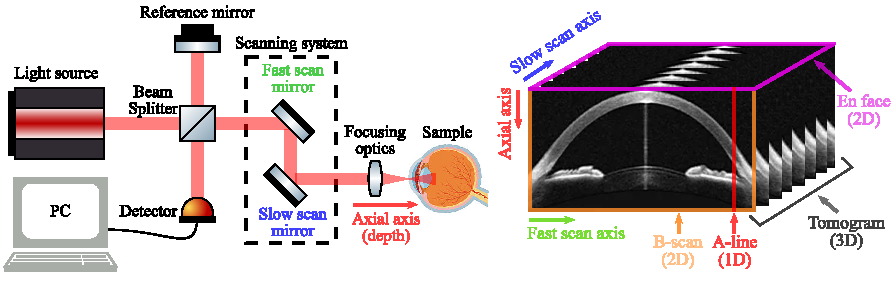
\includegraphics[width=\textwidth]{Figures/Introduction/OCT_ScanningSchemes.pdf}
    \caption[Schematic of a generic OCT setup based on a Michelson interferometer and illustration of common notation.]{Schematic of a generic OCT setup based on a Michelson interferometer and illustration of common notation used for axial axis, transverse axes (fast/slow scan axes), axial scan (A-line) and cross-sectional images (B-scan, \textit{en face}).}
    \label{fig:OCT_ScanningScheme}
\end{figure}

From this general scheme, OCT technology and theory have evolved and to date there is a wide variety of system configurations with particular advantages in terms of imaging speed, sensitivity, imaging depth, among others~\cite{Fujimoto2015_Introduction}. Nonetheless, the use of an optical system to focus the light into the sample and to collect the backscattered light is common to any OCT system and its properties greatly influence the quality of images, most notably, it determines the lateral resolution, i.e. the resolution in the lateral axes, and it may induce optical aberrations that degrade image quality, similarly to any other optical imaging technique~\cite{Ralston2006_Interferometric, Yasuno2006_Noniterative, Adie2012_Computational}.

\section{Aberrations in OCT}

In most OCT systems, light is focused into the sample, so that lateral resolution is defined by the diffraction-limited spot size of the focused light beam~\cite{Fujimoto2015_Introduction}. Optical aberrations, whether from the optical systems or the sample itself, degrade image quality affecting the visualization of fine structures and limiting the axial range where images appear sharp~\cite{Ralston2006_Interferometric,Zawadzki2005_Adaptiveoptics}. To avoid or reduce impact of aberrations, specialized optical systems are used, for instance, telecentric and achromatic systems correct for spherical and chromatic aberrations~\cite{Hu2015_Optical}.

One of the greatest limitations of optical systems is that in-focus images are only obtained for those planes of the sample that are within the \textit{depth of field} (DoF), defined by the numerical aperture (NA) of the system, while beam divergence causes a resolution loss for planes outside the DoF, producing defocused images~\cite{Yasuno2006_Noniterative, Ralston2006_Interferometric}. In the case of OCT, this means that certain planes of the tomogram will be in-focus and appear sharp, but others are out-of-focus and appear blurred. To avoid this, systems with large DoF of $\sim$0.5 -- 2~mm are commonly used so that imaging axial range is limited by signal attenuation in tissue rather than by the effect of defocus. However, this is achieved at the cost of reducing lateral resolution given its inverse relation with DoF, well-known as lateral-resolution--DoF trade-off. For this reason, it is very common that resolution in the transverse plane is lower than resolution in the axial axis, which depends on the central wavelength and spectral bandwidth of the light source and is independent of the NA~\cite{Fujimoto2015_Introduction}.

In addition to system-induced aberrations, the sample can introduce aberrations with a significant impact to reduce image quality, particularly in ophthalmology given that light beam passes through the eye of the subject and imperfections in the cornea and the lens may induce aberrations~\cite{Walsh1984_Objective, Liang1997_Aberrations}.

Because aberrations affect the raw OCT signal, any subsequent post-processing will be influenced by them as well~\cite{Cense2009_Retinal, Park2020_Angiographic}, such is the case of functional imaging techniques like polarization-sensitive OCT (PS-OCT) which is an extension of OCT for measuring the polarimetric properties of the sample~\cite{deBoer1997_Twodimensional}, and OCT angiography (OCT-A) used for vasculature label-free imaging~\cite{Wang2007_Three}.

High-resolution imaging is a very active research field in OCT since it gives access to additional and more detailed information of the sample, which is important in many applications, for example, in cellular imaging as eye photoreceptors~\cite{Zhang2006_Highspeed}. To obtain high-resolution images, aberration can be corrected with hardware-based adaptive optics (AO)~\cite{Zawadzki2005_Adaptiveoptics} or computational aberration correction (CAC)~\cite{Adie2012_Computational}. In AO, additional hardware is used to correct for wavefront distortions \textit{in situ}. It demands complex optics and system design that limits clinical applicability, yet, it is incapable of compensating the lateral-resolution--DoF trade-off given that each depth demands an individual correction but OA applies a global correction~\cite{Pircher2017_Review}.

CAC operates the complex OCT signal using mathematical models based on the propagation of light to compensate aberrations using an appropriate phase filter~\cite{Ralston2006_Interferometric, Yasuno2006_Noniterative, Adie2012_Computational}. CAC addresses lateral-resolution--DoF trade-off but its major limitation is the reduction of signal strength given that acquired signal is weaker in the presence of aberrations, which is an experimental limitation that, in principle, cannot be corrected in post-processing~\cite{Wu2019_Computed}. Currently, operation of CAC is not possible in all OCT systems due to technical limitations that prevent the acquisition of reliable complex-value tomograms~\cite{Shemonski2014_Stability}.

In this work, we present a method for CAC suitable for most common OCT systems to expand its applicability throughout research and clinical applications, making it possible to correct for optical aberration to improve image quality by post-processing in systems where it was not possible due to technical limitations.

\section{Noise in OCT}

Any contribution to the measured signal apart from the backscattered light, that is the interest of OCT, can be considered as \textit{noise}~\cite{Izatt2015_Theory}. In that sense, \textit{speckle} arising in tissue imaging as a consequence of coherent interference of backscattered light with random phases~\cite{Goodman2007_Speckle}, is not noise in rigorous terms, indeed, speckle is important for several functional imaging applications~\cite{Wang2007_Three, Lee2012_Dynamic, Liu2013_Quantitative}, but in practical terms it causes random fluctuations that hinder visual interpretation~\cite{Schmitt1999_Speckle}. Consequently, speckle reduction while preserving visibility of fine structures is an active area of research in OCT~\cite{Cuartas-Velez2018_Volumetric} and in most coherent imaging techniques, such as synthetic aperture radar (SAR)~\cite{Argenti2013_Tutorial}. For this reason, noise reduction in OCT is generally associated with speckle reduction, but there are multiple sources of strictly speaking noise in the OCT signal induced by the system, that have a relevant impact on imaging features such as the \textit{signal-to-noise ration} (SNR), define as the ratio of the signal power and the noise process variance; the sensitivity, defined as the SNR of a perfect reflector placed in the sample arm; and the dynamic range, defined as the range of SNR observable within a signal acquisition or image~\cite{Izatt2015_Theory, deBoer2003_Improved}. SNR is typically given in decibels (dB) through the logarithmic transformation $\text{SNR}_{\text{dB}} = 10\log_{10}\text{SNR}$. Developments in OCT technology had a significant improvement in sensitivity and current imaging systems achieve sensitivities as high as $\sim$100~dB, meaning that minimum detectable reflectivity in the sample is $\sim$1$\times$10$^{-10}$ times the reflectivity of an ideal reference mirror~\cite{Izatt2015_Theory}. In experimental terms, OCT images span dynamic ranges of 40--60~dB although it depends on the tissue and the system.

Most notable sources of noise in the OCT signal are shot, excess and thermal noise~\cite{deBoer2003_Improved}. \textit{Shot} noise originates from the uncertainty of ``counting'' particles of discrete nature such photons and electrons, and it arises in the detection of the OCT signal that involves photon-electron conversion and digitization. \textit{Excess} noise arises from time fluctuations of the incident intensity, mostly due to fluctuation of the emission of the light source. \textit{Thermal} noise stems from random motion of electrons in conductors. In OCT, noise has been addressed mostly experimentally, and at this points it is possible to achieved shot noise limited detection~\cite{deBoer2003_Improved}. For instance, excess noise suppression is achieved using two detectors in a \textit{balanced} detection scheme where non-interfering light ---that contributes the most to excess noise--- is suppressed. Computational approaches for noise reduction have concentrated in speckle suppression, and most shot noise reduction approaches rely on a straightforward average of multiple frame repetitions~\cite{Baumann2019_Signal}.

Reduction of signal strength due to aberrations have a negative impact in SNR and dynamic range because the collected signal is intrinsically lower in the presence of aberrations than in the aberration-free case, and this is not compensated in CAC techniques. An experimental approach to reduce signal strength loss is to use CAC techniques in systems with an astigmatic beam that provides high signal strength throuhout longer depth than a Gaussian beam, so that aberrations are corrected including the astigmatism induced on purpose~\cite{Adie2012_Computational}.


\section{Problem statement}

Post-processing is important in OCT to obtain images with high resolution and contrast as well as additional useful information of the sample, improving and facilitating study, diagnosis and monitory of diseases. Developing techniques to improve image quality in OCT has been the scope of collaborative projects between the Applied Optics Group at Universidad EAFIT and the Wellman Center for Photomedicine at Massachusetts General Hospital and Harvard Medical School. Results include the development of an useful technique for speckle suppresion~\cite{Cuartas-Velez2018_Volumetric}, as well as the derivation of models for robust estimation of the autocorrelation function of intensity OCT signal~\cite{Uribe-Patarroyo2020_Noise} that is the basis of functional imaging modalities such as angiography~\cite{Wang2007_Three} and flowmetry~\cite{Liu2013_Quantitative}. In parallel, experimental setups have been made, including a lab-made accessible full field OCT system~\cite{Cuartas-Velez2019_Labmade} and a linear-in-wavenumber spectrometer for spectral-domain OCT~\cite{Ruiz-Lopera2018_Design}. In addition, a numerical phase correction algorithm was proposed but, given its iterative structure, processing times are and results are limited unpractical~\cite{Cuartas-Velez2017_Formacion}, however, this initial approach for phase stabilization contributed to ideas and notions that led to the current proposal.

Computational aberration correction is a very active field in OCT to improve image quality in application where aberration have a significant impact and to provide high-resolution images~\cite{Adie2012_Computational, Hillmann2016_Aberrationfree, Kumar2017_Invivo}. Development of CAC techniques has been constrained to system configurations that allow a more reliable and robust measurement of the complex-valued tomogram. CAC techniques are based on a common mathematical model, hence requirements for its application are the same, being phase stability the most relevant requirement~\cite{Shemonski2014_Stability}. \textit{Phase stability} is achieved when there is a constant phase relation between measurements at different lateral locations~\cite{Shemonski2014_Stability}, in other words, when there exists a correlation between measurements.

Acquisition of phase stable tomograms is not straightforward in practical terms given that phase is very sensitive to phase noise that affects phase stability~\cite{Shemonski2014_Stability, Vakoc2005_Phaseresolved}, arising from the imaging system and from the sample itself due to axial motion~\cite{Shemonski2014_Stability-1, Shemonski2014_Threedimensional}. In fact, sample motion artifacts include two effects: the first is a phase jump due to Doppler effect~\cite{Chen1997_Optical, White2003_vivo} and the second is the effective shift of the complex information due to sample displacement. Doppler phase noise is the issue most addressed for CAC given that its impact is, in general, more notable than impact of complex-amplitude shift~\cite{Shemonski2014_Stability-1, Shemonski2014_Threedimensional}, although the impact of each effect is relative to features of the imaging system and the amount of motion~\cite{Shemonski2014_Stability}.

Achieving sufficient phase stability for CAC has restricted its usage to custom system configurations with volumetric phase stability, that in some cases is achieved at the cost of increasing system complexity~\cite{Ginner2018_Holographic, Kumar2013_Subaperture, Hillmann2016_Aberrationfree, Sudkamp2018_Simple}. In phase stable systems, operation of CAO is straightforward and for \textit{in vivo} imaging it is sufficient to correct for phase noise due to sample axial motion using numerical corrections based on reference phase signal, generated by adding a highly reflective surface such as a coverslip, or based on the acquired sample signal~\cite{White2003_vivo, Ralston2006_Phase}. Drawback of correction methods based on reference phase signal is that it demands hardware modifications to add a highly reflective surface in addition to the reference mirror.

Numerical phase stabilization methods based on the sample signal assume that there is phase stability at least along one lateral axis, thus correction is only required along the orthogonal lateral axis~\cite{Shemonski2014_Threedimensional}. This assumption is valid for phase stable systems in which phase instabilities in the tomogram arise from sample motion and only affect one lateral axis, commonly the slow scan axis~\cite{Shemonski2014_Threedimensional}. However, there are common OCT configurations that present phase noise induced in the system, for which current numerical phase corrections are hopeless given that there is not any axis with phase stability~\cite{Vakoc2005_Phaseresolved}. Operation of CAO in such phase unstable configurations rely on hardware modifications to avoid system-induced phase noise, restricting its applicability in research and medical application.

Given the current limitation of standard OCT systems to acquire phase stable tomograms, the proposal of this work is \textit{to develop and experimentally test a post-processing method for optical aberration correction in phase unstable tomograms, with no need for hardware modifications or specialized configurations, hence enabling operation of CAC for image quality improvement in system unsuitable for it so far, more specifically, in raster scan wavelength-swept source OCT systems.}

In addition, we also aim to address other important issues in CAC, in regard to the SNR reduction in aberrated tomograms due to signal strength loss, as well as the motion artifacts affecting the complex amplitude, not only the phase.

\newpage
\section{Objectives}
\vspace{\baselineskip}
\subsection{General objective}

To correct optical aberrations in optical coherence tomography with phase unstable systems using post-processing.

\subsection{Specific objectives}

\begin{itemize}
    \item To establish the state-of-art of computational aberration correction in optical coherence tomography.
    \item To identify sources of phase noise and phase correction methods for optical coherence tomography.
    \item To develop a computational method for phase stabilization and aberration correction of tomograms with no intrinsic phase stability.
    \item To test the performance of the method with \textit{ex vivo} and \textit{in vivo} tomograms acquired with typical phase unstable OCT systems.
    \item To identify and analize the possible limitation of the method.
\end{itemize}

\section{Outline of the work}

In this work we present our technique Short Aline-Range Phase-stability adaptive-optics (SHARP) for computational aberration correction in phase unstable systems~\cite{Ruiz-Lopera2020_Computational}, showing successful experimental results using systems with no need for specific hardware that ensure phase stability, in a variety of OCT application ranging from ocular imaging to endoscopic imaging and including \textit{ex vivo} and \textit{in vivo} modalities. SHARP integrates a computational aberration correction technique with numerical phase noise correction to compensate aberrations in phase unstable OCT tomograms, showing particular potential for extending the depth of field to relax the lateral resolution--DoF trade-off.

Additional approaches to address other general drawbacks and limitations of CAC are proposed. Complex noise reduction approaches are presented to countervail the intrinsic reduction of SNR in computational aberration corrected images when compared to experimental aberration-free images. Second, SHARP is extended to admit tomograms affected by complex amplitude shifts due to sample motion for \textit{in vivo} imaging, in addition to Doppler phase term, thus addressing both effects of motion artifacts. Furthermore, an alternative step for correction of spatial-varying aberrations encountered in certain practical scenarios is described. Finally, a strategy to perform computational aberration correction in polarization-sensitive OCT is presented, taking into consideration the particularities of the processing used in this functional imaging technique to properly correct aberrations. Successful computational refocusing of polarimetric properties images of tissue is presented. This is the first integration of computational refocusing in PS-OCT to the best of our knowledge.

There is a particular interest in this work in noise reduction because of its importance not only in CAC but in OCT imaging universally to improve sensitivity and dynamic range. First proposal introduced here for noise reduction is to use a straightforward frequency filter grounded in the context of image deconvolution, that has been used in several imaging modalities, for instance in astronomy, but not in the context of OCT, to the best of our knowledge. In fact, this filter is used for image deconvolution but is not particularly dedicated to noise reduction despite its potential for such purpose.

Second approach is a more sophisticated noise reduction technique that we developed and termed Coherent Tomographic Non-local-means denoising (CTNode). This technique is an adaptation of our previous despeckling technique Tomographic Non-local means despeckling (TNode) where modifications were made in order to address for photon noise in the complex-amplitude tomogram, that is the aim of CTNode, instead of speckle in the intensity tomogram, that is the aim of TNode. Both approaches are based on non-local-means weighted-averaging using statistical properties of its corresponding undesired component, i.e. photon noise or speckle. Experimental results of CTNode are presented in conjunction to SHARP, although applicability of both techniques is independent. CTNode promises to be a more efficient technique than standard approaches based on frames averaging, with potential applications in functional OCT techniques.

\section{Structure of the document}

In this Chapter, a general introduction of OCT was provided to present the problem and the objectives of this work.

In Chapter~\ref{chap:theory}, there is a description of the principle of operation of OCT and the different possible configurations, making emphasis in the level of phase stability that is achieved in each configuration. A mathematical model for the signal of the ``OCT experiment'' is presented from a interferometric perspective and then from a light propagation and image formation perspective. The latter model serves as the basis for the CAC techniques that are then described, followed by a description of phase stability requierment in CAC and phase stabilization techniques, emphasizing in numerical approaches. A simulated tomogram with simple structures generated elsewhere based on the acquisition of the complex OCT signal~\cite{Cuartas-Velez2017_Formacion} is used to illustrate concepts and explanations when required.

Foundation and description of SHARP are given in detail in Chapter~\ref{chap:SHARP}. Results of a proof of concept experiment are presented, in which a cucumber sample presenting remarkable structures was used to acquire tomograms with and without defocus induced intentionally shifting the position of the sample. Furthermore, approaches to address additional important issues in CAC, beside phase stability requirement, are proposed, namely, motion artifacts and spatially-varying aberration correction. Mathematical and conceptual framework of CTNode are also presented in Chapter~\ref{chap:SHARP}, briefly explaining the operation of non-local means algorithm and then deriving its particular operation in CTNode, taking into consideration the origin and statistical description of photon noise in the OCT signal. Results are presented using the simulated noiseless tomogram mentioned previously.

Experimental validation of the methods is presented in Chapter~\ref{chap:results} for a variety of samples, systems and applications, including \textit{ex vivo} and \textit{in vivo} imaging in ophthalmic, endoscopic and dermatologic OCT. Aberration correction with SHARP is demonstrated in anterior segment imaging of swine eye \textit{ex vivo}, endoscopic OCT of swine airway \textit{in vivo}, and skin imaging of human hand dorsal \textit{in vivo} with motion artifacts. Furthermore, it is showed that integration of SHARP and resolution-preserving despeckling technique TNode dramatically improves image quality in comparison to the raw tomograms. Also, noise reduction with CTNode is demonstrated in conjunction with SHARP in anterior segment imaging and independent in human retina imaging \textit{in vivo}, showing a significant noise floor reduction. Additionally, operation of SHARP in PS-OCT based on Stokes processing is demonstrated in the anterior segment of an excised swine eye, showing successful defocus correction in polarimetric parameters of tissue, In each demonstration, a discussion and analysis of the methods and the results are given, highlighting the capabilities and drawbacks.

Finally, conclusions in regard to results and objectives of the work are discussed in Chapter~\ref{chap:conclusions}, as well as possible further steps in the context of noise reduction and computational aberration correction in OCT.